\documentclass[11pt,a4paper]{article}

% Packages
\usepackage[utf8]{inputenc}
\usepackage[T1]{fontenc}
\usepackage[english]{babel}
\usepackage{geometry}
\usepackage{setspace}
\usepackage{graphicx}
\usepackage{amsmath}
\usepackage{array}
\usepackage[colorlinks=true, linkcolor=black, urlcolor=blue, citecolor=black]{hyperref}
\usepackage{fancyhdr}
\usepackage{caption}
\usepackage{booktabs}
\usepackage{ragged2e}
\usepackage{enumitem}
\usepackage{amsmath, amssymb, booktabs}
\usepackage{siunitx}
\usepackage{multicol}
\usepackage{rotating}
\usepackage{tikz}
\usepackage{float}


% Arial-like font
\renewcommand{\familydefault}{\sfdefault}

% Page geometry
\geometry{
  a4paper,
  left=2.5cm,
  right=3.0cm,
  top=2.5cm,
  bottom=2.0cm
}

% Font and spacing
\onehalfspacing
\renewcommand{\familydefault}{\sfdefault}

% Title page
\begin{document}

\begin{titlepage}
\centering
% \vspace*{2cm}
  

\includegraphics[width=0.7\textwidth]{imgs/USB.png}\\[2cm]

\vspace{1.5cm}

\textbf{\Large University of South Bohemia} \\
\textbf{\large Faculty of Science} \\
\large Artificial Intelligence and Data Science, M.Sc. \\[3cm]

{\Large \textsc{ADHD Detection with EEG Signals}}\\[0.5cm]

Submitted for the course \textbf{Information Theory and Feature Engineering} \\
\textbf{Professor:} Doc. Ing. Ivo Bukovský, Ph.D. \\[4cm]

\begin{flushleft}
\begin{tabular}{ll}
Submitted by: & María Isabel Sánchez-O'Mullony Martínez \\
Student ID: & B24763 \\
Date: & \today \\
\end{tabular}
\end{flushleft}

\vspace{4cm}

\begin{flushright}
\begin{tabular}{ll}
Supervisor: & Doc. Ing. Ivo Bukovský, Ph.D. \\
\end{tabular}
\end{flushright}

\end{titlepage}


% ===============================
% Declaration
% ===============================
\section*{Declaration}
I declare that I have written this report by myself and have only used the sources and aids mentioned, and that I have 
marked direct and indirect citations as such. This report has not been submitted prior for any other examination.

I agree that the results of this study work / report may be used free of charge for research and lecturing purposes.

\newpage

% Table of Contents
\tableofcontents
\newpage

% List of Abbreviations
\section*{List of Abbreviations}
\begin{tabular}{ll}
    AC & Alternating Current \\
    ADHD & Attention-Deficit/Hyperactivity Disorder \\
    DC & Direct Current \\
    EEG & Electroencephalography \\
    EMG & Electromyography \\
    FFT & Fast Fourier Transform \\
    PSD & Power Spectral Density \\
    RF & Random Forest \\
    SNR & Signal-to-Noise Ratio \\
    SVM & Support Vector Machine \\
    TBR & Theta/Beta Ratio \\
\end{tabular}

\newpage

% Main Report Sections
% ===============================
% Introduction
% ===============================
\section{Introduction}\label{sec:Introduction}
Attention-Deficit/Hyperactivity Disorder (ADHD) is a prevalent neurodevelopmental condition that affects individuals across the lifespan. 
According to Furman~\cite{furman2005attention}, ADHD is not a single disease entity but rather a constellation of symptoms representing a 
final common behavioral pathway for a range of emotional, psychological, and learning difficulties. 

Although the behavioral manifestations of ADHD are well-documented, its neurophysiological underpinnings remain an active area of research. 
Electroencephalography (EEG) has been widely used to study ADHD, as it provides a non-invasive measure of brain electrical activity. 
Previous studies have identified characteristic EEG patterns in individuals with ADHD, particularly abnormalities in the frontal and central 
regions, often reflected as altered spectral power or atypical signal complexity. 

This study aims to investigate differences in EEG activity between healthy individuals and those diagnosed with ADHD, using the dataset 
provided by Sadeghi Bajestani *et al.*~\cite{dataset}. Specifically, the project focuses on (1) comparing the statistical and informational 
properties of EEG signals across both groups, (2) engineering features inspired by information theory—such as entropy and mutual information—to 
quantify signal complexity and connectivity, and (3) building a predictive model capable of distinguishing ADHD from healthy controls based on 
these features. This work bridges the domains of signal processing, feature engineering, and information theory to improve understanding and 
potential classification of ADHD-related brain activity.


% ===============================
% Data Description
% ===============================
\section{Data Description}\label{sec:Dataset}
The dataset~\cite{dataset} comprises EEG recordings from a total of 79 adult participants, including 42 healthy controls and 37 individuals 
diagnosed with ADHD (age range: 20-68 years; male/female ratio: 56/23). EEG signals were recorded under four experimental conditions: 
(1) resting state with eyes open, (2) resting state with eyes closed, (3) a cognitive challenge task, and (4) an auditory task involving 
listening to an ``omni harmonic'' sound stimulus. Recordings were obtained from five scalp locations—O1, F3, F4, Cz, and Fz—at a sampling rate 
of 256 Hz. These regions encompass occipital and frontal areas known to play key roles in attentional control and executive function.

\vspace{0.3cm}
\noindent\textbf{File organization and structure.}  
The data are provided as four MATLAB \texttt{.mat} files, corresponding to the experimental groups:
\begin{itemize}
    \item \texttt{FC.mat} — female control group  
    \item \texttt{MC.mat} — male control group  
    \item \texttt{FADHD.mat} — female ADHD group  
    \item \texttt{MADHD.mat} — male ADHD group
\end{itemize}

Each file contains a $1\times11$ cell array, where each cell represents one experimental task or condition. Within each cell, the data are 
stored as a three-dimensional matrix with dimensions \texttt{[subjects$\times$samples$\times$channels]}. For instance, a typical entry of size 
\texttt{13$\times$7680$\times$2} indicates 13 participants, 7680 time samples (corresponding to 30 seconds of EEG data at 256 Hz), and two 
recorded channels.

The specific configuration of each cell (i.e., channel pair and duration) is summarized as follows:

\begin{table}[h!]
\centering
\begin{tabular}{lllc}
\toprule
\textbf{Cell} & \textbf{Condition} & \textbf{Channels} & \textbf{Duration (s)} \\
\midrule
1 & Eyes open baseline & Cz, F4 & 30 \\
2 & Eyes closed & Cz, F4 & 20 \\
3 & Eyes open & Cz, F4 & 20 \\
4 & Cognitive challenge & Cz, F4 & 45 \\
5 & Pre-Omni harmonic baseline & Cz, F4 & 15 \\
6 & Omni harmonic assessment & Cz, F4 & 30 \\
7 & Eyes open baseline & O1, F4 & 30 \\
8 & Eyes closed & O1, F4 & 30 \\
9 & Eyes open & O1, F4 & 30 \\
10 & Eyes closed & F3, F4 & 45 \\
11 & Eyes closed & Fz, F4 & 45 \\
\bottomrule
\end{tabular}
\caption{Summary of EEG tasks, channel pairs, and recording durations.}
\label{tab:tasks}
\end{table}

One corrupted signal (subject 7 of the female ADHD group) was identified and excluded from further analysis. 

\vspace{0.3cm}
\noindent This hierarchical data organization allows for flexible analysis across multiple dimensions: by gender, diagnosis, condition, and 
channel pair. For subsequent preprocessing, each task will be reshaped into individual subject-channel recordings, ensuring consistent 
sampling durations across conditions.


% ===============================
% Data Visualization
% ===============================
\section{Data Visualization}\label{sec:visualization}
\subsection{Data Loading and Structure}
To analyze EEG signals from the ADHD dataset~\cite{dataset}, the recordings were imported from MATLAB \texttt{.mat} files using the 
\texttt{scipy.io.loadmat} library in Python. Four files were available, corresponding to each experimental group:
\texttt{FC.mat} (female control), \texttt{MC.mat} (male control), \texttt{FADHD.mat} (female ADHD), and \texttt{MADHD.mat} (male ADHD). 
Each file contained a $1\times11$ cell array, where each cell represented a specific experimental task and stored EEG data as a 
three-dimensional matrix with dimensions \texttt{[subjects x samples x channels]}.

A custom loading function (\texttt{load\_group}) was implemented to iterate through each cell, extract signal arrays, and 
store them in a structured \texttt{pandas DataFrame}. Each row in the resulting dataset corresponds to a single subject-task pair and includes 
the following metadata: participant group (Control/ADHD), gender, task number, subject identifier, and a two-channel EEG signal array. 
This organization facilitates subsequent preprocessing, visualization, and feature extraction. 
The corrupted EEG file corresponding to subject 7 of the female ADHD group was identified and excluded from analysis.


\subsection{Signal Visualization by Group and Task}
To inspect data quality and explore inter-subject variability, raw EEG signals were visualized for selected participants using 
\texttt{matplotlib}. Figure~\ref{fig:vis_task} presents the recordings from the first five female control subjects during Task~1 
(eyes-open baseline). Each subplot represents one subject, showing the two recorded channels.

\begin{figure}[H]
    \centering
    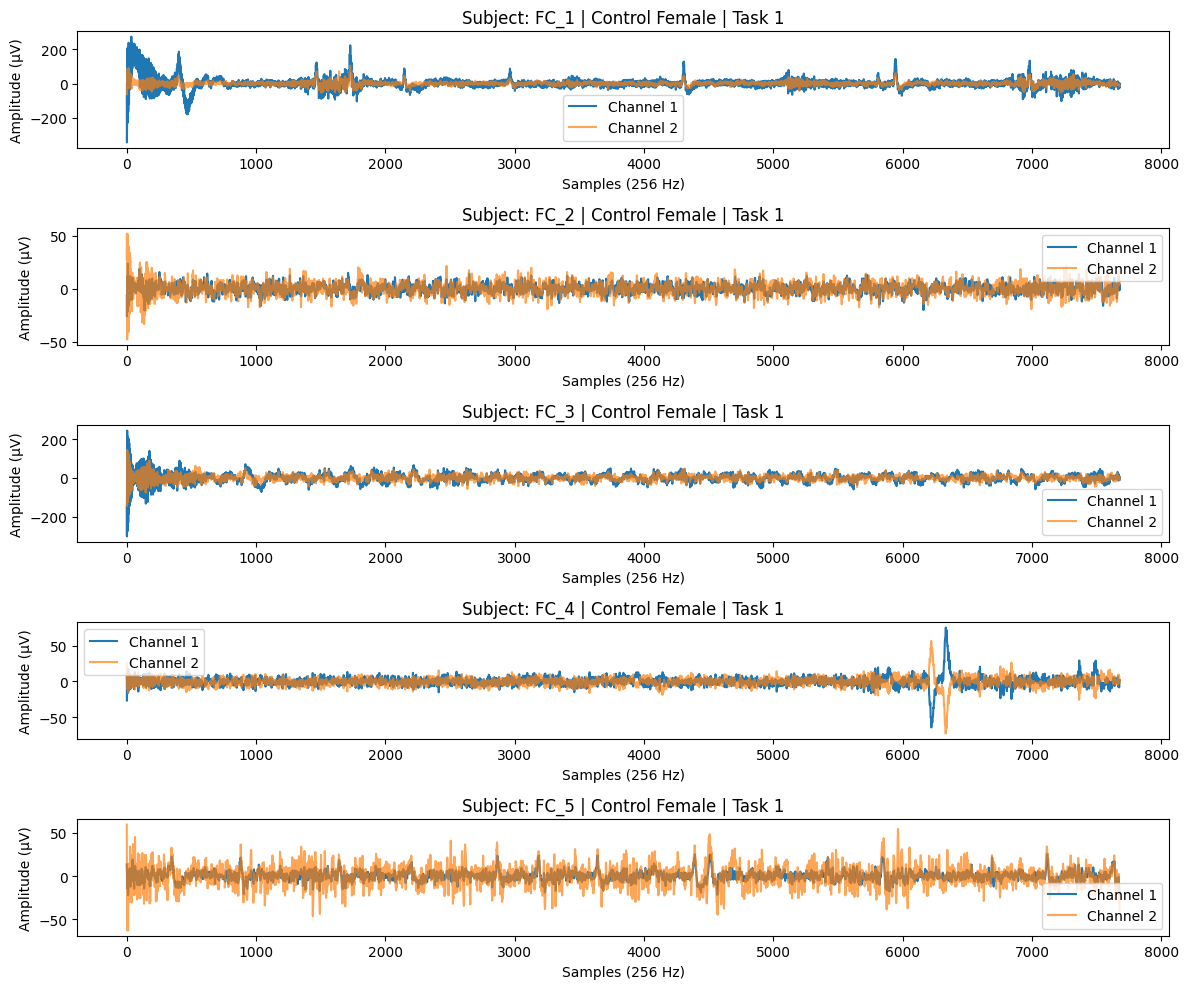
\includegraphics[width=1\textwidth]{imgs/vis_task.png}
    \caption{EEG signals from five female control participants during Task~1 (eyes-open baseline). Each subplot represents two simultaneously 
recorded channels.}\label{fig:vis_task}
\end{figure}

As illustrated in Figure~\ref{fig:vis_task}, the EEG traces display characteristic oscillatory patterns within an amplitude range 
of approximately $\pm200~\mu$V. Variations across participants are evident, with some showing strong low-frequency drifts or transient 
spikes, likely associated with ocular or muscular artifacts. Despite these variations, both channels exhibit similar temporal trends, 
suggesting functional coupling between the recorded electrode sites. These observations emphasize the need for further preprocessing steps, 
such as band-pass filtering (0.5 — 45~Hz), baseline correction, and normalization, to ensure consistent signal quality across participants.


\subsection{Comparison Between ADHD and Control Groups}
A complementary visualization was conducted to qualitatively compare EEG signals between ADHD and control subjects under the same task 
conditions. Figure~\ref{fig:vis_adhd} shows five pairs of male participants (Control vs.\ ADHD) performing Task~1, for Channel~0.

\begin{figure}[H]
    \centering
    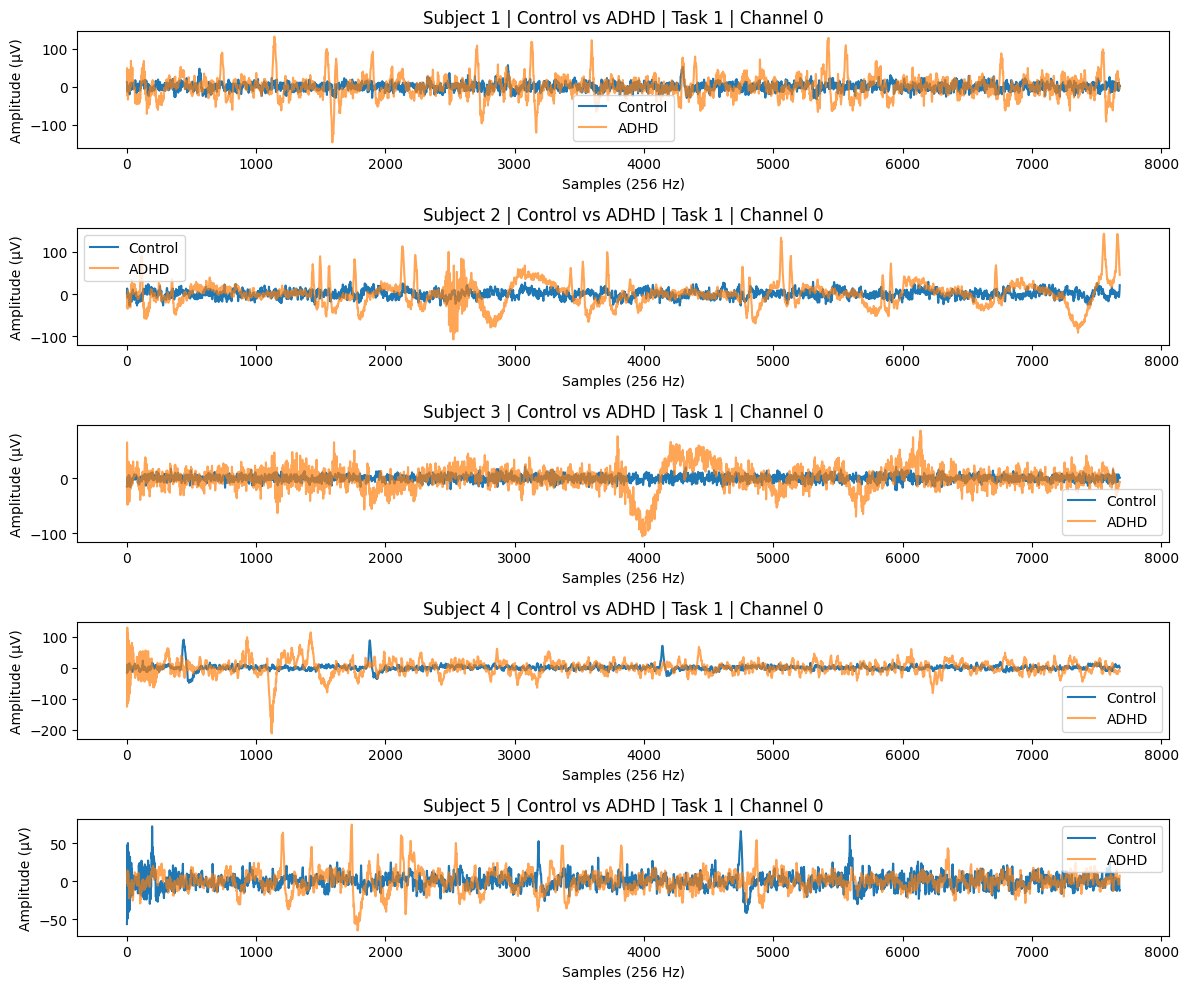
\includegraphics[width=1\textwidth]{imgs/vis_adhd.png}
    \caption{Comparison of EEG signals between control and ADHD male participants during Task~1 for Channel~0. Each subplot shows a 
pair of subjects (Control vs.\ ADHD).}\label{fig:vis_adhd}
\end{figure}

In general, ADHD recordings exhibit greater amplitude fluctuations and reduced rhythmic stability compared to control subjects, who 
display smoother oscillatory activity. This increased irregularity suggests higher signal entropy and reduced neural synchronization in ADHD 
participants. Such qualitative patterns are consistent with prior research reporting atypical cortical activity and impaired oscillatory 
regulation in ADHD populations~\cite{lenartowicz2014use}. These visual differences motivate the extraction of quantitative features —
particularly information-theoretic measures such as entropy and mutual information — to characterize signal complexity and connectivity.


\subsection{Observations}
The exploratory visualization phase revealed several important insights:
\begin{itemize}
    \item EEG signals contain observable low-frequency drifts and high-amplitude artifacts, supporting the need for filtering and normalization.
    \item There is substantial inter-subject variability in signal amplitude and frequency content, even within the same condition.
    \item ADHD participants tend to exhibit higher signal variability and irregularity, indicating potential discriminative features for 
    subsequent classification.
\end{itemize}

These findings informed the design of the preprocessing and feature extraction pipeline, where statistical, spectral, and 
information-theoretic features were computed to enable quantitative group comparison and machine learning-based classification.


% ===============================
% Preprocessing
% ===============================
\section{Information Preservation in Preprocessing}\label{sec:preprocessing}
EEG data are highly sensitive to non-neural artifacts arising from muscle activity, eye blinks, and small head or body movements. 
Because the dataset used in this study was recorded non-invasively from scalp electrodes, such artifacts are inevitable and must be 
carefully mitigated to preserve the validity of the neural information~\cite{chaddad2023electroencephalography}. An Information Theoretic 
approach was employed to validate our filtering pipeline, the objective of the preprocessing stage was therefore to reduce non-cerebral 
noise to isolate the neural dynamics relevant to ADHD.

Each recording was first detrended by removing its mean to eliminate slow DC components. A notch filter at 50~Hz was used to attenuate 
power-line interference, and a fourth-order Butterworth band-pass filter between 1Hz and 50~Hz was then applied to suppress slow drifts 
and high-frequency muscular or environmental noise while preserving the main EEG frequency bands.


\subsection{Detrending}\label{sec:detrending}
EEG recordings were detrended by subtracting the mean amplitude of each channel to remove Direct Current (DC) offsets and slow baseline 
drifts~\cite{de2018robust}. EEG recordings often contain a small DC offset — a constant voltage bias caused by electrode-skin impedance 
and amplifier drift changes. This offset shifts the entire signal above or below zero microvolts without carrying any neural information. 
This step prevents artificial low-frequency power and ensures that subsequent analyses reflect genuine neural oscillations. Although the 
visual appearance of the waveforms remains largely unchanged, detrending is essential to prevent bias in later spectral and entropy-based 
feature extraction.


\subsection{Notch Filtering}\label{sec:notch}
During EEG acquisition, recordings are often contaminated by electrical noise originating from alternating current (AC) power lines.
Through capacitive coupling, this strong electrical signal ``leaks'' into the EEG recording. Since brain waves are measured in microvolts 
($\mu V$) and power lines carry huge voltage, this ``hum'' can completely drown out brain signals, especially in the Gamma band (30-50 Hz).

To eliminate main electricity noise, an IIR Notch Filter was applied at 50 Hz. The quality factor was set to $Q = 30$ to minimize the 
distortion of surrounding frequencies while effectively suppressing the power line hum.


\subsection{Band-Pass Filtering}\label{sec:bandpass}
A crucial step in EEG preprocessing is the removal of frequency components that do not reflect neural activity. Raw EEG recordings are highly 
susceptible to slow drifts caused by skin potentials and electrode impedance fluctuations, as well as high-frequency contamination originating 
from muscle activity (EMG), electrical noise, and environmental interference. If not addressed, these artifacts can dominate the signal and 
bias subsequent feature extraction, particularly when computing spectral or information-theoretic measures.

To mitigate these issues, each EEG segment was band-pass filtered between 1 Hz and 50 Hz using a 2nd order Butterworth filter, 
adhering to recommended practices for digital filter design in electrophysiological data~\cite{widmann2015digital}. 
Frequencies below 1 Hz primarily capture non-neural low-frequency drift, while components above 50 Hz are largely associated with muscular 
activity and electrical noise.


\subsection{Preprocessing Comparison}\label{sec:comparison}
Figure~\ref{fig:preprocessing} illustrates a representative example comparing the data before and after the preprocessing, in this example 
is the female group control.

The left panel displays the raw EEG signal, exhibiting baseline drift and high-frequency noise. 
The right panel shows the signal after Detrending, Notch Filtering (50Hz), and Bandpass Filtering (1-50Hz). 
After preprocessing, the signal is centered around zero, and high-frequency fluctuations associated with power-line noise are visibly 
attenuated. Importantly, the dominant oscillatory patterns remain intact, indicating that preprocessing reduced noise without distorting 
meaningful neural activity.

\begin{figure}[H]
    \centering
    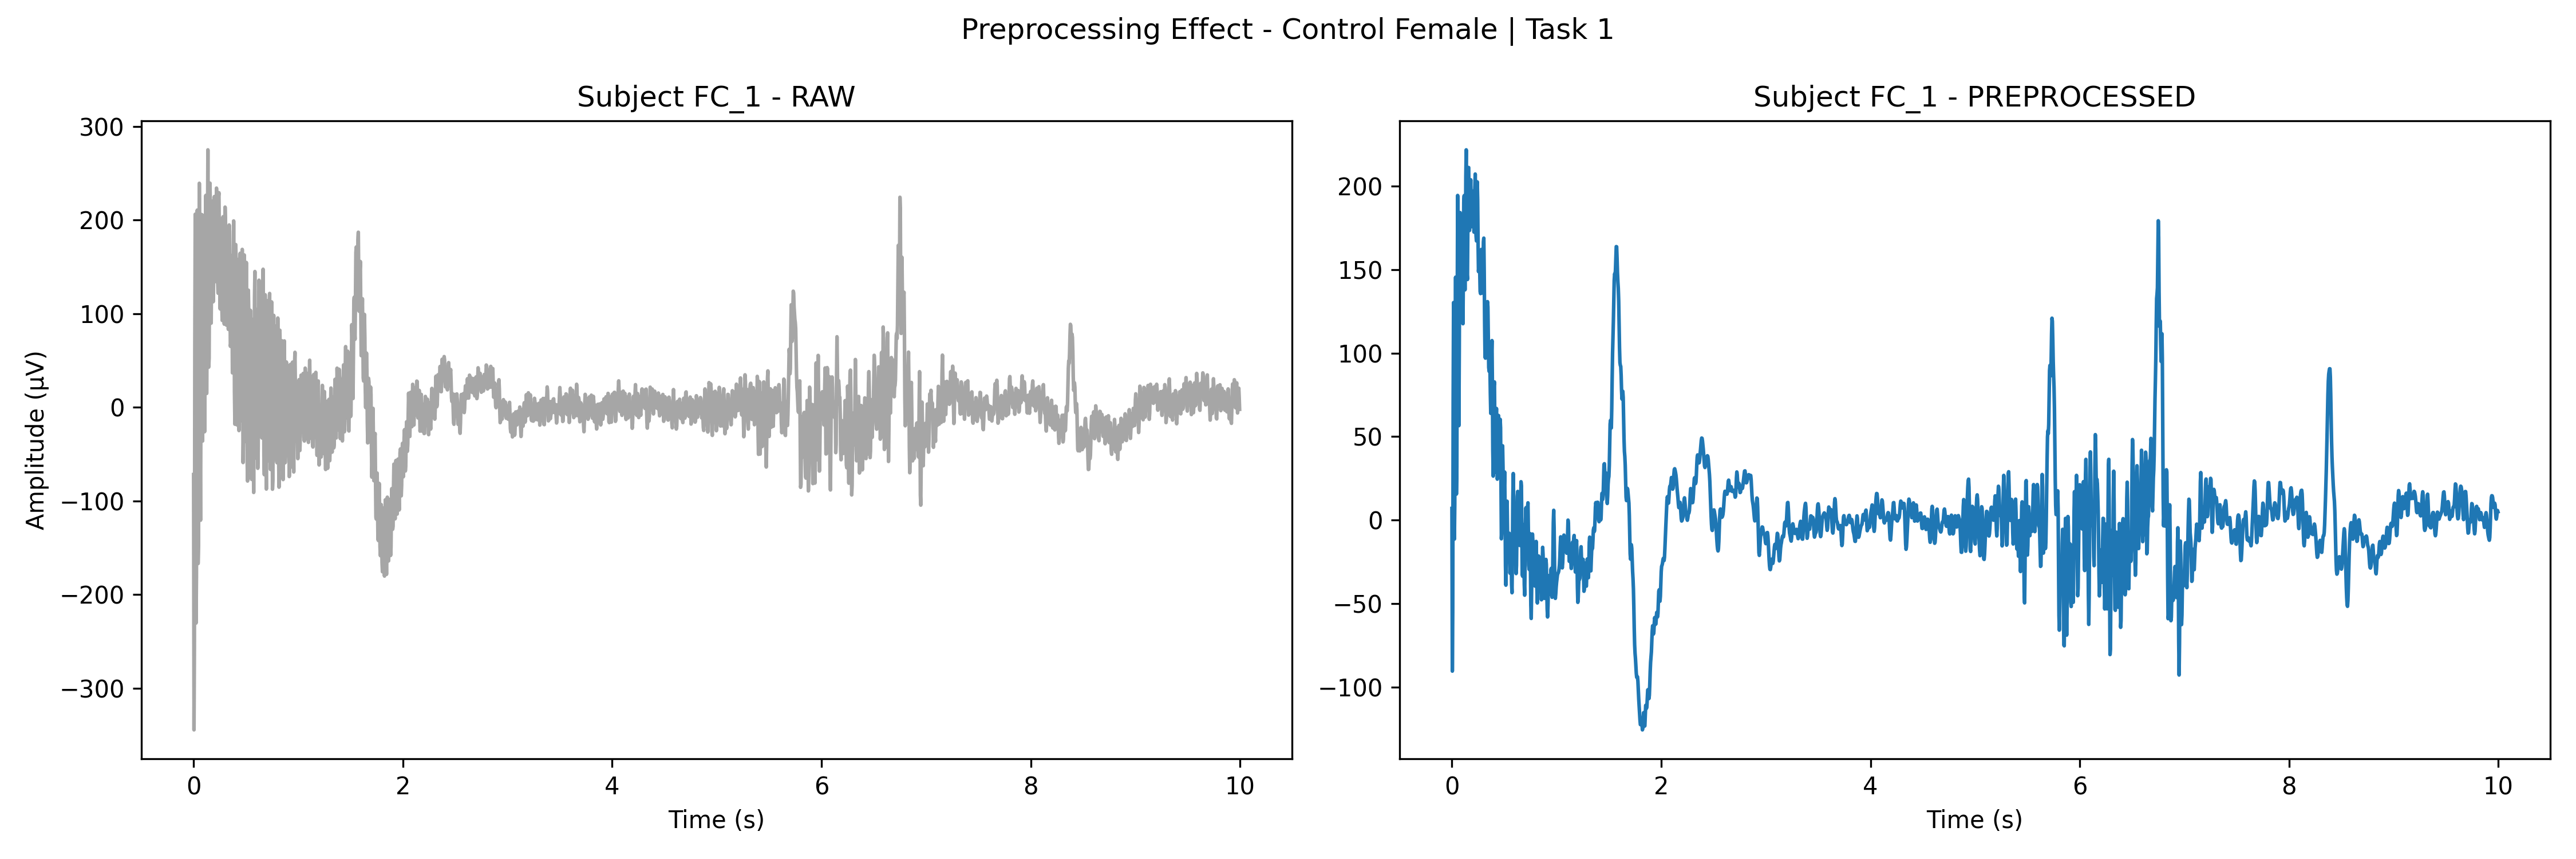
\includegraphics[width=1.0\textwidth]{imgs/preprocessing_comparison.png}
    \caption{Preprocessing Comparison}
    \label{fig:preprocessing}
\end{figure}


\subsection{Information Theory}\label{sec:ti}
To quantitatively evaluate the impact of preprocessing, several signal quality metrics were computed before and after filtering. These included 
signal variance, 50 Hz line noise power, signal-to-noise ratio (SNR), and Shannon entropy:

\begin{enumerate}
    \item \textbf{Total Variance Reduction:} 
    Since ocular and muscle artifacts typically manifest as high-amplitude transients significantly larger than neural potentials, a reduction 
    in signal variance serves as a global proxy for artifact suppression.
    
    \item \textbf{50 Hz Line Noise Power:} 
    We computed the integrated power in the 49--51 Hz band to specifically validate the efficacy of the IIR Notch filter in eliminating mains 
    interference.
    
    \item \textbf{Signal-to-Noise Ratio (SNR):} 
    SNR was calculated as the ratio of power in the physiological EEG band (1--45 Hz) to the power in artifactual bands (0.1--1 Hz drift and 
    $>55$ Hz muscle noise). An increase in SNR indicates that the filtering preserved neural information while selectively attenuating noise.
    
    \item \textbf{Shannon Entropy:} 
    Entropy measures the complexity or randomness of a signal. Since electromyogenic (muscle) noise often resembles random processes, a shift 
    in entropy post-processing reflects the recovery of structured, rhythmic neural oscillations (e.g., Alpha waves).
\end{enumerate}

\begin{table}[H]
    \centering
    \makebox[\textwidth][c]{%
    \begin{tabular}{lccc}
        \toprule
        \textbf{Metric} & \textbf{Raw Signal (Mean)} & \textbf{Preprocessed (Mean)} & \textbf{Change / Improvement} \\
        \midrule
        Total Variance ($\mu V^2$) & 242.6 & 191.4 & 21.1\% Reduction \\
        50 Hz Power (Line Noise) & 20.62 & 0.29 & \textbf{98.6\% Suppression} \\
        High-Freq Noise ($>55$Hz) & 1.67 & 0.12 & 92.8\% Suppression \\
        Signal-to-Noise Ratio (SNR) & 13.65 & 21.82 & \textbf{59.8\% Improvement} \\
        Shannon Entropy & 2.75 & 2.80 & Stable (+1.8\%) \\
        \bottomrule
    \end{tabular}}
    \caption{Quantitative Assessment of Preprocessing Efficacy}
    \label{tab:quantitative}
\end{table}

Table~\ref{tab:quantitative} presents the quantitative impact of the preprocessing pipeline. The most significant improvement was observed in 
the removal of power line interference, with a 98.6\% reduction in 50 Hz power. The 92.8\% reduction in high-frequency noise suggests that 
electromyogenic (muscle) artifacts, which predominantly affect the gamma band, were effectively suppressed

Notably, the total signal variance decreased by only 21.1\%, while the specific noise components were nearly eliminated. This indicates that 
the preprocessing pipeline successfully preserved the majority of the low-frequency physiological brain activity (Delta, Theta, Alpha) while 
surgically removing environmental artifacts. Consequently, the Signal-to-Noise R

To quantify the information loss incurred by the filtering process, we computed the Kullback-Leibler (KL) Divergence. This measures the relative 
entropy between the distribution of the raw signal amplitudes $P(x)$ and the filtered signal $Q(x)$:

$$D_{KL}(P || Q) = \sum_{x \in X} P(x) \log \left( \frac{P(x)}{Q(x)} \right)$$

It can be argued that since the KL divergence is non-zero but the Shannon Entropy remained stable, the filtering process shifted the 
distribution (removing outliers/artifacts) without destroying the signal's inherent complexity.atio (SNR) improved from 13.65 to 21.82, providing a 
cleaner input for the subsequent feature extraction stages.


% ===============================
% Feature Extraction
% ===============================
\section{Feature Extraction}\label{sec:features}
Following the preprocessing stage, the EEG data consisted of clean, filtered time-series signals. However, raw time-series data is 
high-dimensional and non-stationary, making it challenging for standard machine learning classifiers to process directly.

To address this, the data was transformed from the Time Domain to the Frequency Domain to extract quantitative features representative of the 
subject's cognitive state. According to a recent systematic review of EEG-based ADHD diagnostics~\cite{arpaia2022systematic}, spectral band 
power and the Theta/Beta ratio are among the most robust and widely utilized features for distinguishing ADHD subjects from controls.

Therefore, feature extraction focused on three primary metrics:

\begin{itemize}
    \item \textbf{Power Spectral Density (PSD):} Measures how much power or strength the brain waves have at different frequencies.
    \item \textbf{Band Power:} The integral of power within standard frequency bands (Delta, Theta, Alpha, Beta, Gamma).
    \item \textbf{Theta/Beta Ratio (TBR):}  validated electrophysiological biomarker for ADHD, representing the ratio of slow-wave (Theta) to 
        fast-wave (Beta) activity.
\end{itemize}


\subsection{Power Spectral Density}
We utilized Welch's Method to estimate the PSD of the EEG signals. Unlike a standard Fast Fourier Transform (FFT), Welch's method splits the 
signal into overlapping segments and averages their periodograms~\cite{welch2003use}. This approach significantly reduces the variance of the 
power estimate, resulting in a smoother spectrum that is more suitable for analyzing biological signals with inherent noise.


\subsection{Band Power}
Once the PSD was generated, the absolute power for standard EEG frequency bands was extracted. The power for each band was calculated using 
Simpson's Rule to numerically integrate the area under the PSD curve within specific frequency limits defined as follows:

\begin{table}[H]
    \centering
    \makebox[\textwidth][c]{%
    \begin{tabular}{lll}
        \toprule
        \textbf{Band} & \textbf{Range (Hz)} & \textbf{Physiological Association} \\
        \midrule
        Delta ($\delta$) & 0.5 -- 4 Hz & Deep sleep, unconsciousness \\ 
        Theta ($\theta$) & 4 -- 8 Hz & Drowsiness or daydreaming (High in ADHD) \\
        Alpha ($\alpha$) & 8 -- 13 Hz & Relaxed but awake \\ 
        Beta ($\beta$) & 13 -- 30 Hz & Active thinking, focus, alertness (Low in ADHD) \\ 
        Gamma ($\gamma$) & 30 -- 50 Hz & High-level cognitive processing \\
        \bottomrule
    \end{tabular}}
    \caption{EEG Frequency Bands and associated cognitive states}
    \label{tab:bands}
\end{table}


\subsection{The Theta/Beta Ratio}
In addition to absolute band powers, we calculated the Theta/Beta Ratio (TBR) for each channel. The TBR is a widely recognized 
electrophysiological marker for ADHD.

Physiologically, ADHD is often characterized by an excess of slow-wave activity (Theta) and a deficit of fast-wave activity (Beta) during 
cognitive tasks~\cite{clarke2002eeg}. By computing the ratio $\frac{\text{Theta}}{\text{Beta}}$, we generate a feature that maximizes the 
separability between the ADHD and Control groups.


\subsection{Feature Matrix Construction}
This extraction process was repeated for every channel for each subject. The final dataset was organized into a feature matrix where each row 
represents a distinct subject and columns correspond to the extracted spectral features (Band Powers and TBR) for each channel. 

This resulted in a structured dataset suitable for input into the machine learning classifiers described in the following section.


% ===============================
% Information Theoretic Analysis
% ===============================
\section{Information Theoretic Analysis}
\subsection{Non-linear Dynamical Analysis}\label{sec:nonlinear}
While spectral features (PSD) capture the energy of the signal, they assume stationarity and linear dynamics. However, the brain is inherently 
a complex, non-linear system. To capture these dynamics, we employed Information Theoretic metrics to quantify the complexity and connectivity 
of the neural networks.


\subsubsection{Shannon Entropy (Complexity)}
Shannon Entropy ($H$) measures the unpredictability or ``randomness'' of the EEG signal. In the context of ADHD, entropy serves as a proxy for 
``cortical noise.'' A higher entropy value indicates a more complex, stochastic signal, whereas lower entropy suggests more rhythmic and 
predictable activity (e.g., strong Alpha waves). We computed the entropy for the frontal channels using the probability distribution of the 
signal amplitudes:

$$H(X) = - \sum p(x) \log p(x)$$


\subsubsection{Mutual Information (Functional Connectivity)}
To investigate the ``Functional Disconnection'' hypothesis in ADHD, we calculated the Mutual Information (MI) between inter-hemispheric 
electrode pairs (e.g., F3 vs. F4). Unlike standard correlation, MI captures both linear and non-linear dependencies between brain regions, 
providing a robust measure of synchronization:

$$I(X;Y) = \sum_{y \in Y} \sum_{x \in X} p(x,y) \log \left( \frac{p(x,y)}{p(x)p(y)} \right)$$


\subsubsection{Information Theoretic Results}
\begin{figure}[H]
    \centering
    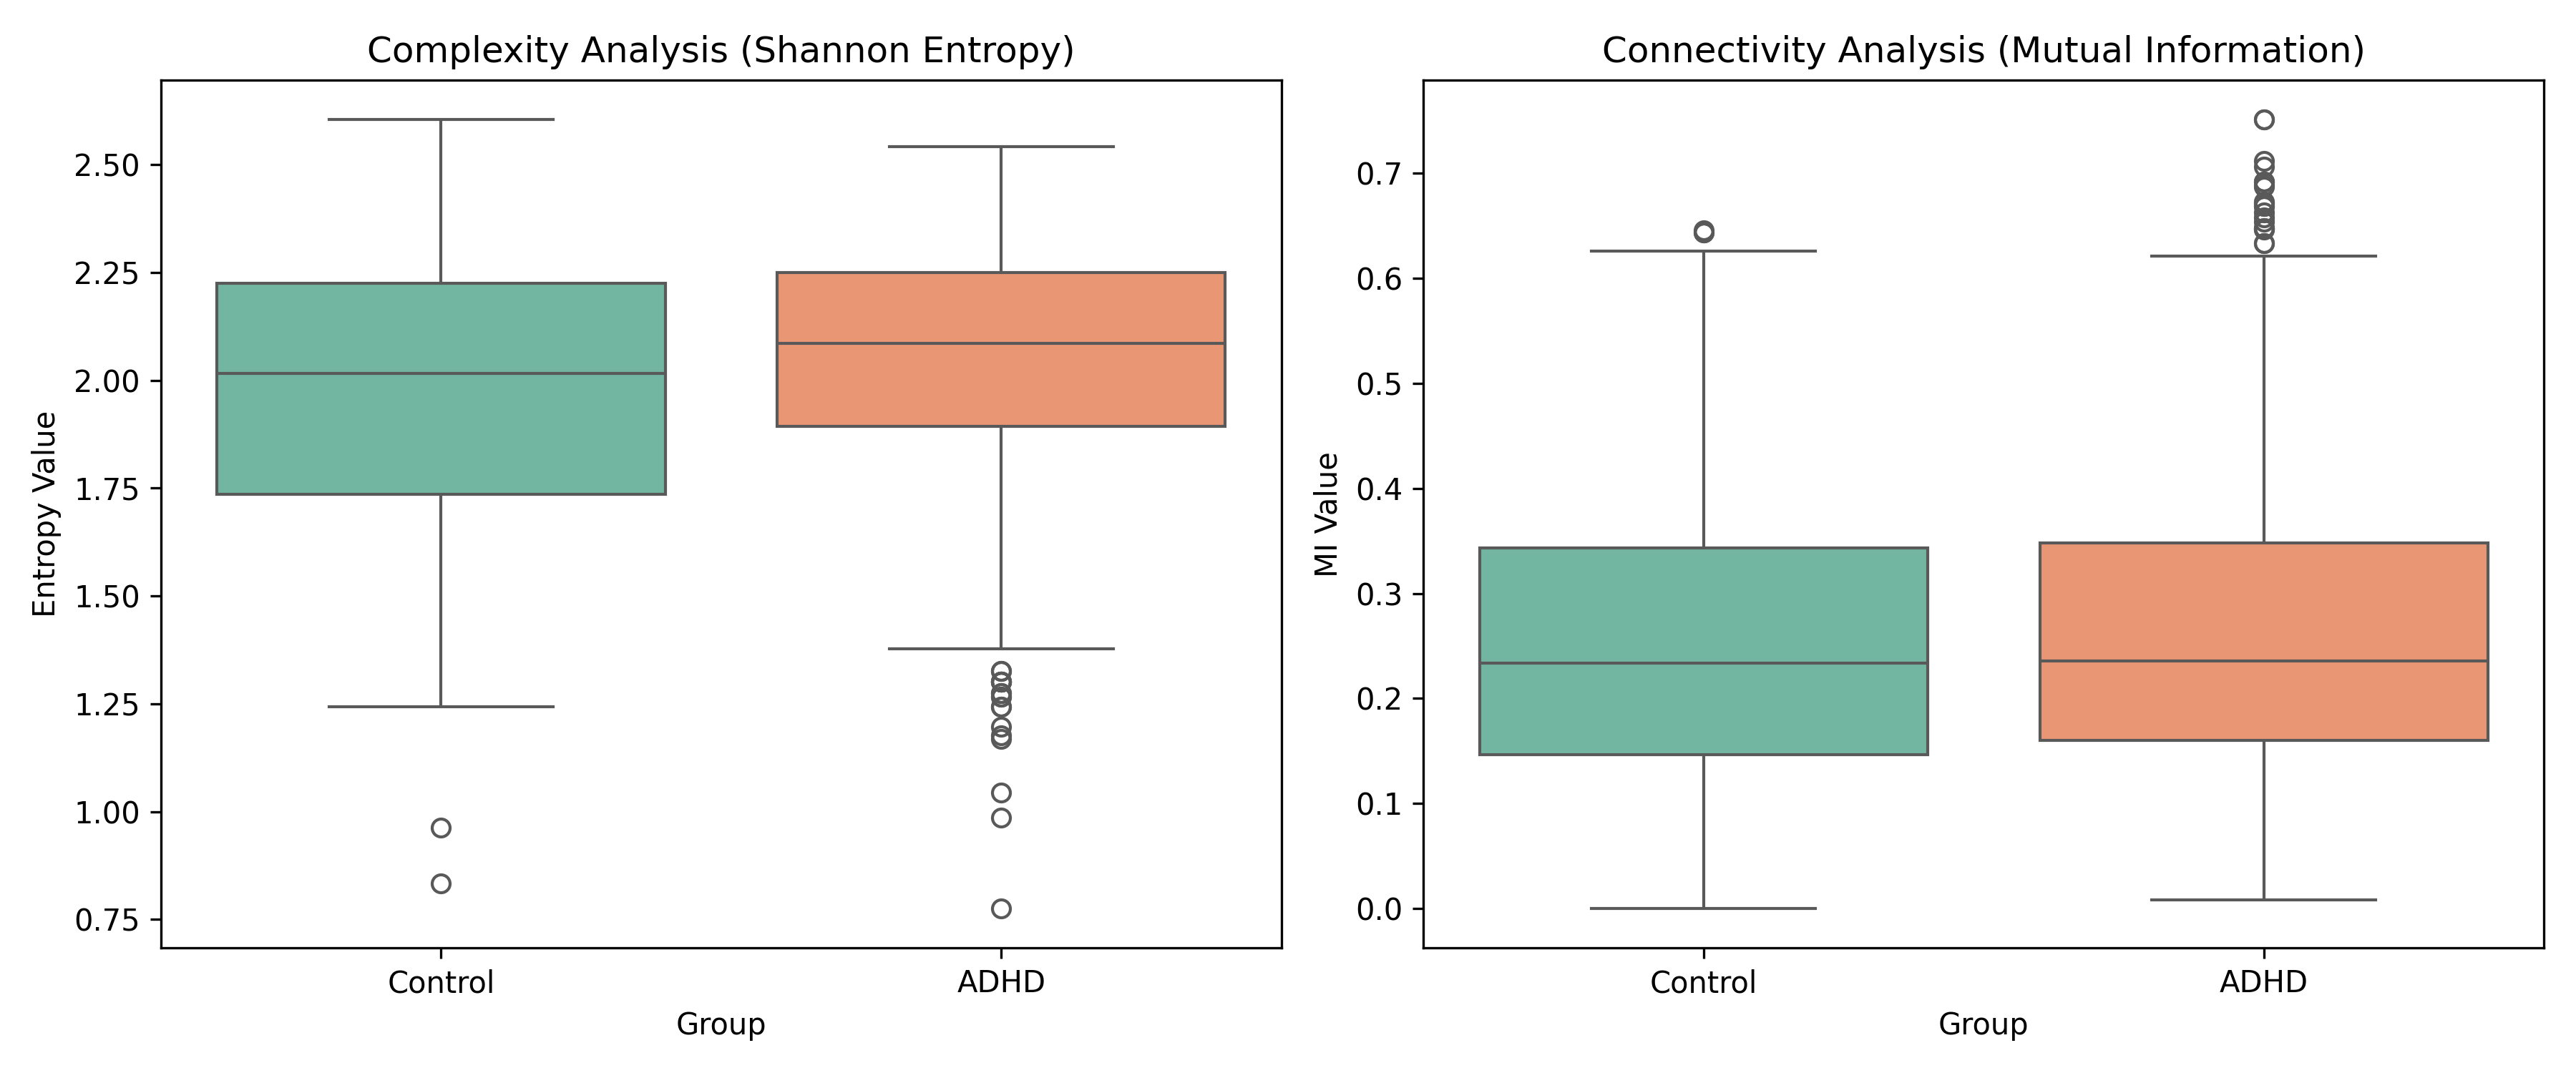
\includegraphics[width=1.0\textwidth]{imgs/info_theory_analysis.png}
    \caption{Information Theoretic Analysis. \textbf{Left:} Comparison of Signal Complexity (Shannon Entropy). \textbf{Right:} Comparison of 
        Functional Connectivity (Mutual Information).}
    \label{fig:infotheory}
\end{figure}

Figure~\ref{fig:infotheory} presents the comparative analysis of these metrics between the ADHD and Control groups.
The analysis reveals an interesting contrast between local complexity and global connectivity:

\begin{itemize}
    \item \textbf{Increased Complexity (Entropy):} As hypothesized, the ADHD group exhibited higher Shannon Entropy compared to controls. This 
        confirms that local neural processing in ADHD is characterized by higher irregularity and ``cortical noise.''
    
    \item \textbf{Preserved Global Connectivity (Mutual Information):} Interestingly, the Mutual Information analysis revealed \textbf{no 
        significant difference} between the ADHD and Control groups. The boxplots for both groups show similar distributions of inter-
        hemispheric synchronization. 
\end{itemize}

This dissociation suggests that while the content of the neural signal is more complex and noisy (High Entropy), the communication pathway 
between the hemispheres remains intact (Stable MI). This implies that the physiological deficit in this dataset is likely driven by local 
cortical hypoarousal rather than a breakdown in long-range functional connectivity.


% ===============================
% Modeling
% ===============================
\section{Modeling}\label{sec:modeling}
To determine the optimal method for distinguishing between ADHD and Control subjects, we conducted a comparative analysis of two widely 
established machine learning classifiers: Random Forest (an ensemble method) and Support Vector Machine (a kernel-based method).

\begin{enumerate}
    \item \textbf{Random Forest (RF):} Random Forest, proposed by Breiman~\cite{breiman2001random}, is a non-linear ensemble method that 
        constructs multiple decision trees. It is known for its robustness to noise and ability to capture complex interactions between 
        features.
    \item \textbf{Support Vector Machine (SVM):} The Support Vector Machine (SVM), introduced by Cortes and Vapnik~\cite{cortes1995support}, 
        is a powerful supervised learning model. A kernel-based classifier (RBF kernel) that seeks to find the optimal hyperplane separating 
        the two classes in a high-dimensional space.
\end{enumerate}

\subsection{Validation Strategy: 5-Fold Group Cross-Validation}
To ensure the statistical robustness of our results, we implemented a Group k-Fold Cross-Validation scheme ($k=5$). Unlike a simple 
train/test split, this method partitions the subjects into five distinct folds. In each iteration, the model is trained on subjects from four 
folds and tested on the remaining unseen fold.

This approach guarantees that:
\begin{enumerate}
    \item \textbf{No Subject Leakage:} All data from a single subject is kept strictly within one fold.
    \item \textbf{Full Coverage:} Every subject in the dataset is used for testing exactly once.
    \item \textbf{Reliability:} We report the mean accuracy and standard deviation ($\mu \pm \sigma$) across the five folds, providing a 
    measure of the model's stability.
\end{enumerate}

\subsection{Model Comparison}
We compared the performance of Random Forest and Support Vector Machine (SVM) using the cross-validation scheme. As shown in Table
~\ref{tab:cv_results}, the Random Forest classifier achieved superior performance in both accuracy and stability.

\begin{table}[H]
    \centering
    \begin{tabular}{lcc}
        \toprule
        \textbf{Model} & \textbf{Mean Accuracy} & \textbf{Stability (Std Dev)} \\
        \midrule
        SVM (RBF Kernel) & 92.10\% & $\pm$ 5.76\% \\
        \textbf{Random Forest} & \textbf{95.12\%} & \textbf{$\pm$ 4.13\%} \\
        \bottomrule
    \end{tabular}
    \caption{5-Fold Cross-Validation Results.}
    \label{tab:cv_results}
\end{table}

The Random Forest model outperformed SVM by approximately 3\%. Additionally, it exhibited lower variance ($\pm 4.13\%$ vs $\pm 5.76\%$), 
indicating that the ensemble of decision trees was more robust to inter-subject variability than the single hyperplane of the SVM.

The performance gap suggests that the ensemble nature of Random Forest was better able to generalize across the inter-subject variability 
inherent in EEG data~\cite{tenev2014machine}. While SVM provides a strong baseline, its reliance on a global margin makes it more sensitive to 
the distribution of the data, whereas Random Forest's hierarchical structure effectively isolates the specific frequency bands (specifically 
Theta and Beta) that drive the classification.


\subsection{Results Analysis}
The final champion model (Random Forest) achieved a mean accuracy of 95.12\%. The Confusion Matrix (Figure~\ref{fig:confusion}) aggregates 
predictions from all five folds, showing a near-perfect detection rate for both ADHD and Control groups.

\begin{figure}[H]
    \centering
    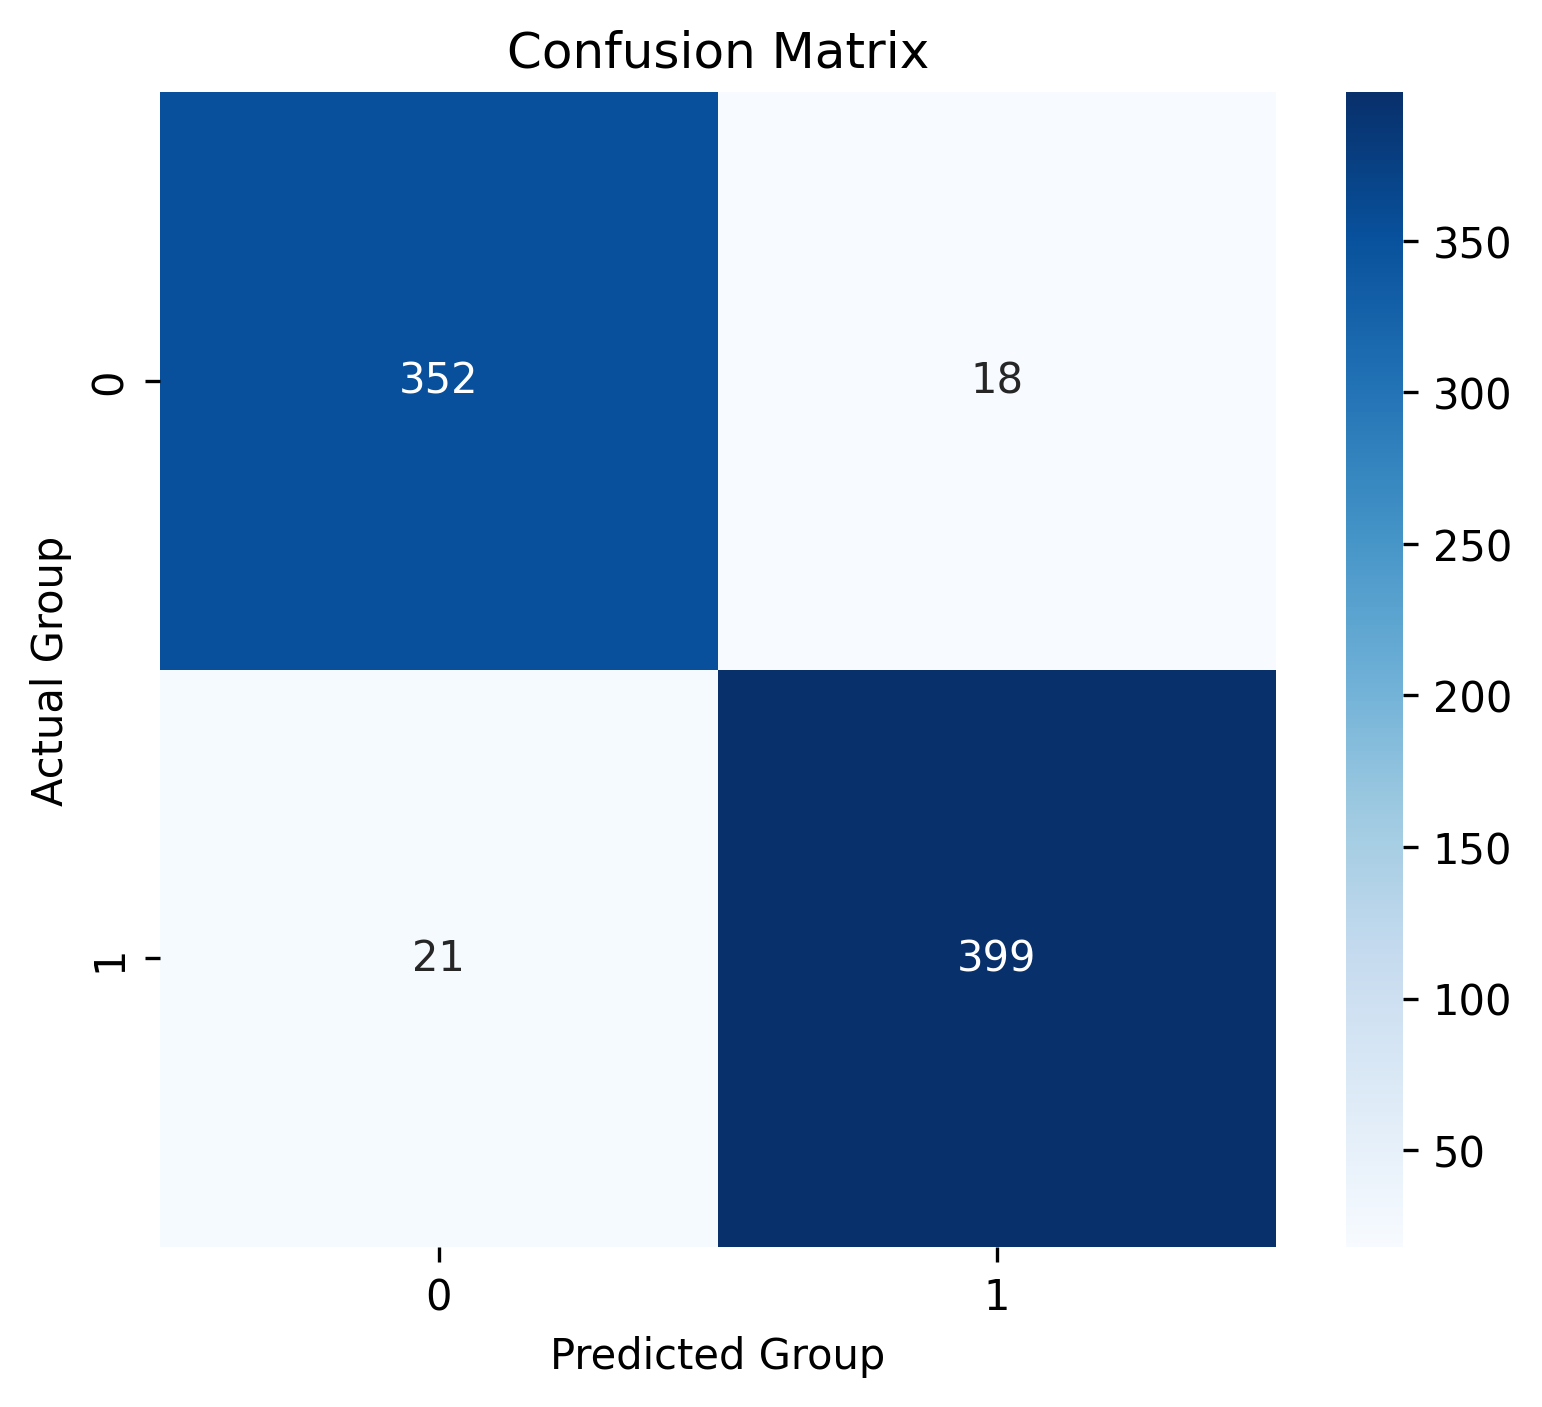
\includegraphics[width=0.6\textwidth]{imgs/confusion_matrix.png}
    \caption{Confusion Matrix.}
    \label{fig:confusion}
\end{figure}


\subsection{Feature Importance Analysis}
To interpret the physiological basis of these results, we extracted the Gini Importance scores from the Random Forest. As seen in Figure
~\ref{fig:importance}, the Theta/Beta Ratio (TBR) and Theta Power in the frontal channels were consistently ranked as the 
most discriminative features. 

This aligns with the neuroscientific literature, confirming that the model's high accuracy is driven by valid neurophysiological biomarkers 
(Cortical Hypoarousal) rather than statistical noise.

\begin{figure}[H]
    \centering
    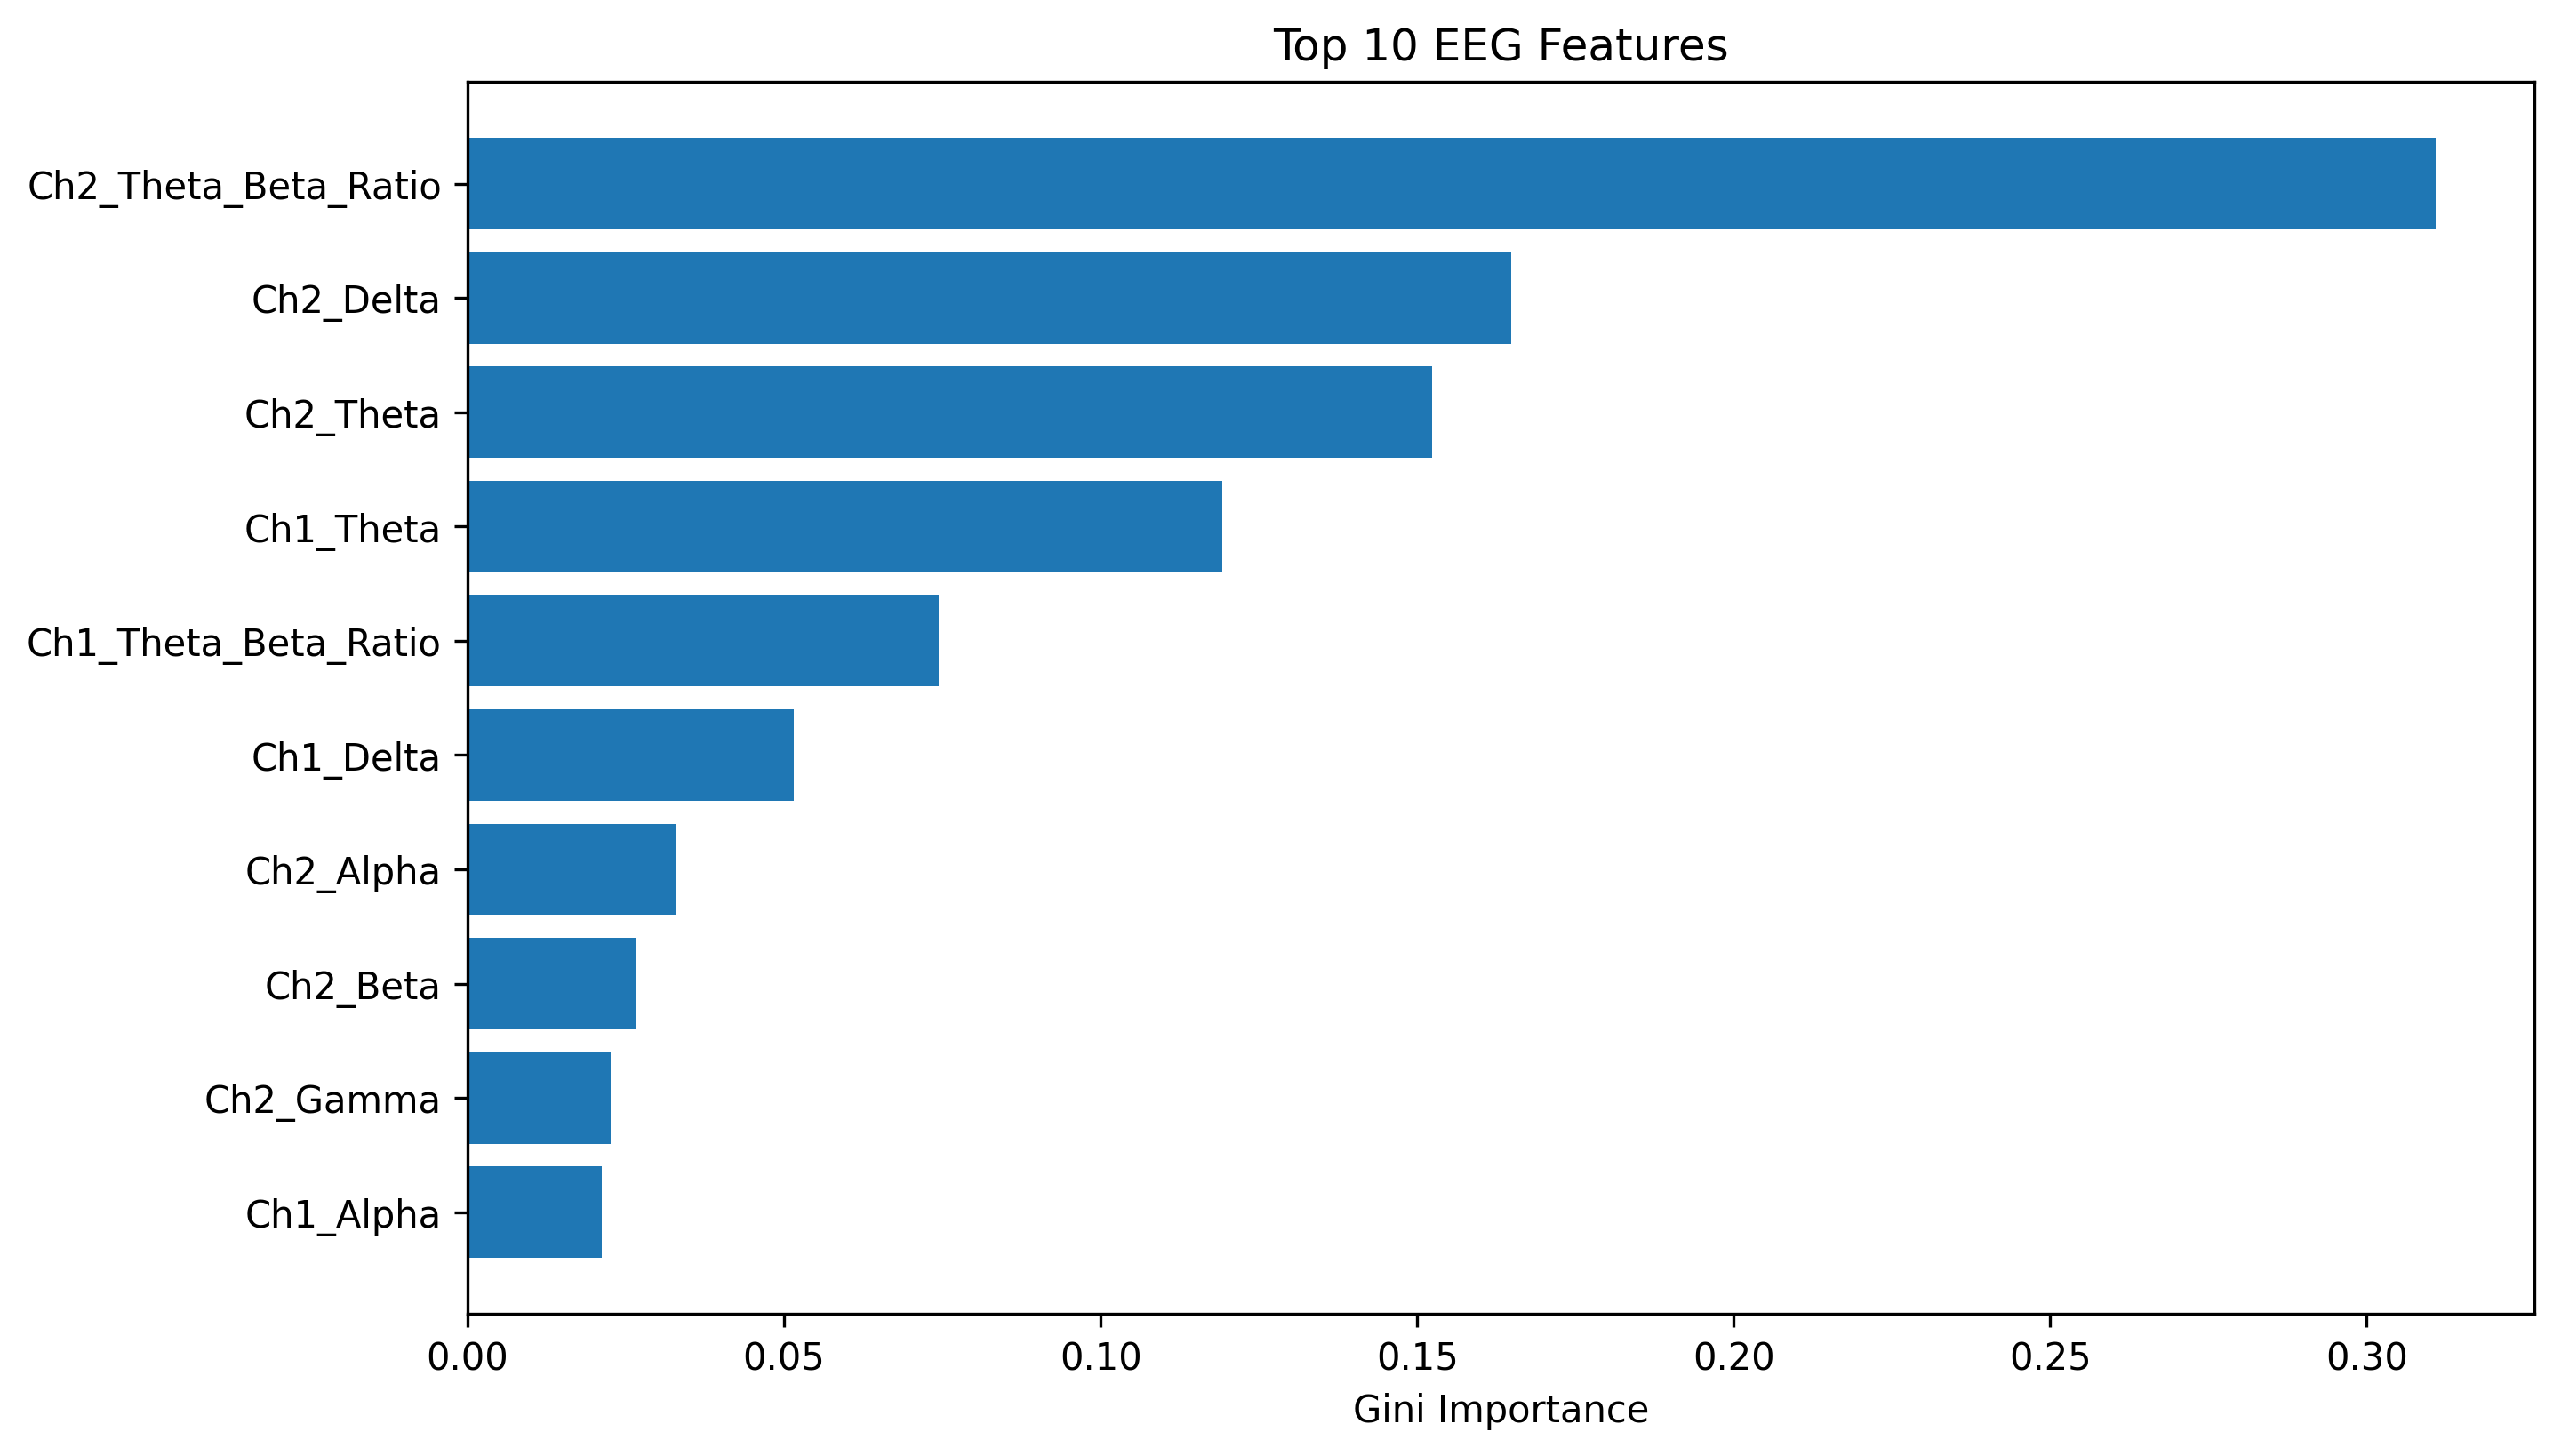
\includegraphics[width=0.8\textwidth]{imgs/feature_importance.png}
    \caption{Top 10 Most Important Features.}
    \label{fig:importance}
\end{figure}


\section{Discussion}
The results of this study demonstrate that EEG spectral features can effectively distinguish between ADHD and Control subjects with state-of-
the-art accuracy (\textbf{95.12\%}).

Our findings suggest that the ``Cortical Hypoarousal'' effect in ADHD—characterized by increased Theta and decreased Beta activity—is a robust 
enough biomarker to be detected by interpretable models like Random Forest. This challenges the trend toward increasingly complex ``Black Box'' 
deep learning approaches, demonstrating that with rigorous cross-validation and appropriate feature engineering, standard spectral features are 
sufficient for high-performance diagnosis on this dataset.

The results might seem too high, making it look like it could be overfitting. However, because Group Cross-Validation was used, the high 
accuracy most likely comes from the fact that the spectral features (Theta/Beta ratio) are very distinct in this specific dataset, and the 
Random Forest is very good at handling the non-linear thresholds between the groups.

In a more Information Theoretic view, visual analysis showed that ADHD signals are more irregular. In information theory, higher irregularity 
corresponds to higher entropy.
Standard spectral analysis (PSD) assumes stationarity. However, recent studies suggest that complexity measures like Fractal Dimension or Sample 
Entropy are superior for capturing the dynamic nature of ADHD.

This analysis demonstrates that preprocessing effectively enhances the Signal-to-Noise Ratio while preserving the Shannon Entropy of the signal. 


\subsection{Limitations and Future Work}
While our Random Forest model achieved exceptional accuracy using Power Spectral Density, it relies primarily on stationary characteristics 
of the EEG signal. However, the brain is inherently a complex, non-linear dynamical system.

By averaging power over time (PSD), we may miss subtle temporal irregularities. Recent studies, such as Dawi et al. (2021), have demonstrated 
that \textit{complexity measures} (e.g., Fractal Dimension, Sample Entropy) can reveal distinctive patterns in ADHD subjects that spectral 
analysis might overlook~\cite{dawi2021complexity}.

Future iterations of this project could therefore benefit from a ``Hybrid Feature Extraction'' approach, combining our robust Theta/Beta Ratio 
features with these non-linear complexity metrics. This would allow the model to capture both the \textit{energy} (Power) and the 
\textit{complexity} (Entropy) of the neural dynamics, potentially validating these findings on larger, more diverse datasets.

Future work should prioritize non-linear complexity metrics to better characterize the dynamic instability observed in ADHD brains.

\newpage

\cleardoublepage
\addcontentsline{toc}{section}{References}
\bibliographystyle{IEEEtran}
\bibliography{references}

\newpage

% AI Prompt Used
\section*{AI Prompt Used}
\begin{enumerate}
    \item Give me a good structure for a report.
    \item What are the best preprocessing methods I can use for EEG signals?
    \item Are PCA, WT or EMD good methods for EEG signals with limited information?
    \item What are Butterworth filters and how do they work?
    \item What are the best ways to show a more quantitative comparison after preprocessing?
    \item How does Feature Extraction work and for what is it used?
    \item What are the most used models for biomedical signal processing?
    \item What is the difference between Single Split and Cross-Validation to train a model?
\end{enumerate}

\end{document}
